\subsection{信号的分解方法}

信号有多种方法可以进行分解:
\begin{itemize}
    \item 直流分量 + 交流分量
    \item 偶分量 + 奇分量
    \item 实部分量 + 虚部分量
    \item 脉冲分量
    \item 基于正交分量的分解
\end{itemize}

\begin{definition}[信号的直流/交流分解]
    设 $f(t)$ 为一个信号,定义其\bd{直流分量}为
    \begin{align*}
        f_{\text{AC}} = \lim_{T \to \infty}\frac{1}{T}\int_{T/2}^{-T/2}f(t)\D{t},
    \end{align*}
    其\bd{交流分量}为
    \begin{align*}
        f_{\text{AC}}(t) = f(t) - f_{\text{DC}}.
    \end{align*}
\end{definition}

\begin{definition}[信号的奇/偶分解]
    设 $f(t)$ 是一个信号,定义其\bd{奇分量}为
    \begin{align*}
        f_{\text{o}}(t) = \text{Od}[f(t)] = \frac{f(t) - f(-t)}{2},
    \end{align*}
    其\bd{偶分量}为
    \begin{align*}
        f_{\text{e}}(t) = \text{Ev}[f(t)] = \frac{f(t) + f(-t)}{2}.
    \end{align*}
\end{definition}

\begin{definition}[信号的实部/虚部分解]
    设 $f(t)$ 是一个信号,定义其\bd{实部分量}为
    \begin{align*}
        f_{\text{r}}(t) = \re[f(t)] = \frac{f(t) + f^*(t)}{2},
    \end{align*}
    其\bd{虚部分量}为
    \begin{align*}
        f_{\text{i}}(t) = \im[f(t)] = \frac{f(t) - f^*(t)}{2\mathi}.
    \end{align*}
\end{definition}

\begin{definition}[信号的脉冲分解]
    信号的\bd{脉冲分解}是指,信号可以近似地被表示为一组矩形脉冲的和的形式。
    设 $f(t)$ 是一个信号,定义其在 $t_1$ 处的矩形脉冲可以表示为如图 \ref{fig:rect-pulse-decomposition} 所示的函数:
    \begin{align*}
        f_{t_1}(t) = f(t_1)[u(t - t_1) - u(t - t_1 - \Delta t_1)],
    \end{align*}
    则 $f(t)$ 可以表示为
    \begin{align*}
        f(t) \approx \sum_{t_1 = -\infty}^{+\infty}f_{t_1}(t)
            = \sum_{t_1 = -\infty}^{+\infty}f(t_1)[u(t - t_1) - u(t - t_1 - \Delta t_1)].
    \end{align*}
    \begin{figure}[H]
        \centering
        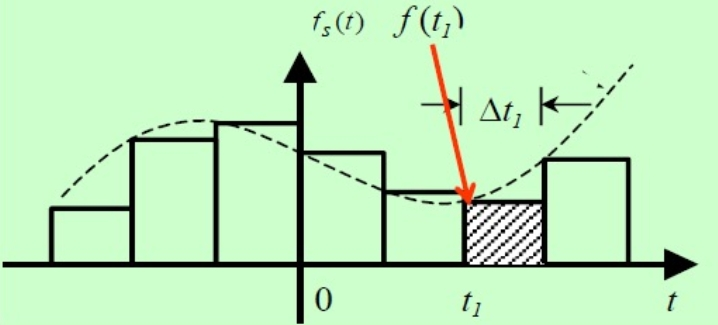
\includegraphics[width=0.5\textwidth]{chap2/img/rect-pulse-decomposition}
        \caption{$f(t)$ 的脉冲分解}
        \label{fig:rect-pulse-decomposition}
    \end{figure}
\end{definition}

\begin{note}
    信号的直流/交流分解、奇/偶分解、实部/虚部分解的结果是\bd{唯一}的,脉冲分解是结果是\bd{近似}的。
\end{note}
